\documentclass[10pt,a4paper]{jsarticle}
\usepackage{listings,jlisting}
\usepackage{fancyhdr}
\usepackage{lastpage}
\usepackage[dvipdfmx]{graphicx,color}
\usepackage{comment}

\lhead{プログラミング実習IIレポート(第7回)}
\rhead{学籍番号:201811433 氏名:西田 直人}
\cfoot{\thepage/\pageref{LastPage}}

\pagestyle{fancy}

\title{プログラミングII実習レポート課題第7回}
\author{西田直人}

\begin{document}
%\markright{プログラミング実習1Aレポート(第1回) 学籍番号:201811433 氏名:西田直人}
%\maketitle
\begin{center}
{\LARGE プログラミング実習IIレポート課題第7回} \\
\large
西田直人 \\ 2019年1月18日
\end{center}
\normalsize
\section{課題7-1}

\subsection{source}
\noindent a.
\lstinputlisting[basicstyle=\ttfamily\footnotesize,frame=single,breaklines=tr\
  ue,caption=Makefile1a]{Makefile1a}
\lstinputlisting[basicstyle=\ttfamily\footnotesize,frame=single,breaklines=tr\
  ue,caption=a7-1.c]{a7-1.c}
\lstinputlisting[basicstyle=\ttfamily\footnotesize,frame=single,breaklines=tr\
  ue,caption=aLoadSave.c]{aLoadSave.c}
\lstinputlisting[basicstyle=\ttfamily\footnotesize,frame=single,breaklines=tr\
  ue,caption=aStructs.c]{aStructs.c}
\lstinputlisting[basicstyle=\ttfamily\footnotesize,frame=single,breaklines=tr\
  ue,caption=headerA.h]{headerA.h}


b.
\lstinputlisting[basicstyle=\ttfamily\footnotesize,frame=single,breaklines=tr\
  ue,caption=Makefile1b]{Makefile1b}
\lstinputlisting[basicstyle=\ttfamily\footnotesize,frame=single,breaklines=tr\
  ue,caption=b7-1.c]{b7-1.c}
\lstinputlisting[basicstyle=\ttfamily\footnotesize,frame=single,breaklines=tr\
  ue,caption=gauss.c]{gauss.c}


\subsection{result}
\noindent 7-1a.

\begin{comment}
\begin{figure}[htbp]
  \begin{minipage}{0.25\hsize}
    \begin{center}
    
\includegraphics[width=30mm]{color4x4_ascii.jpg}
    \end{center}
    \caption{入力画像:ASCII カラー画像}
    \label{fig:sutehage}
  \end{minipage}
  \begin{minipage}{0.25\hsize}
    \begin{center}
      
\includegraphics[width=30mm]{checker4x4_ascii.jpg}
    \end{center}
    \caption{入力画像:ASCII グレースケール画像}
    \label{fig:sutehage}
  \end{minipage}
  \begin{minipage}{0.25\hsize}
    \begin{center}
      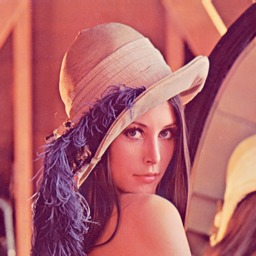
\includegraphics[width=30mm]{lenna256x256binary.jpg}
    \end{center}
    
    \caption{入力画像:Binary カラー画像}
    \label{fig:sutehage}
  \end{minipage}
  \begin{minipage}{0.25\hsize}
    \begin{center}
      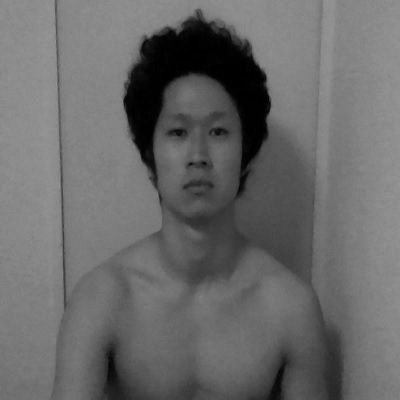
\includegraphics[width=30mm]{sutehage400x400binary.jpg}
    \end{center}
    \caption{入力画像:Binary グレースケール画像}
    \label{fig:sutehage}
  \end{minipage}
\end{figure}
\end{comment}

本当は入力画像の情報も載せていたが、platexの際にオ
ーバーフローを起こすとかバッファが足りないとか怒られて(! Unable to read an ent\
  ire line---bufsize=200000.
  Please increase buf_size in texmf.cnf.
)のせることができなかった。ネットで検索したらsudoを使ってtexmf.cnの内部のbufsi\
zeを書き換えたらいけるっぽかったけど、ルート権限になることができなかった。(s18\
  11433@LC2RR-P010:~/prog2/07/07kadai$ sudo su -
  [sudo] s1811433 のパスワード:
  残念ですが、ユーザー s1811433 は'/bin/su -' を root として LC2RR-P010.u.tsukuba\
  .ac.jp 上で実行することは許可されていません。)



\begin{figure}[htbp]
  
  \begin{minipage}{0.25\hsize}
    \begin{center}
      
      
\includegraphics[width=30mm]{copied_asc_color.jpg}
    \end{center}
    \caption{出力画像:ASCII カラー画像}
    \label{fig:sutehage}
  \end{minipage}
  \begin{minipage}{0.25\hsize}
    \begin{center}
      
      
\includegraphics[width=30mm]{copied_asc_gray.jpg}
    \end{center}
    \caption{出力画像:ASCII グレースケール画像}
    \label{fig:sutehage}
  \end{minipage}
  \begin{minipage}{0.25\hsize}
    \begin{center}
      
      \includegraphics[width=30mm]{copied_bina_color.jpg}
    \end{center}
    \caption{出力画像:Binary カラー画像}
    \label{fig:sutehage}
  \end{minipage}
  \begin{minipage}{0.25\hsize}
    \begin{center}
      
      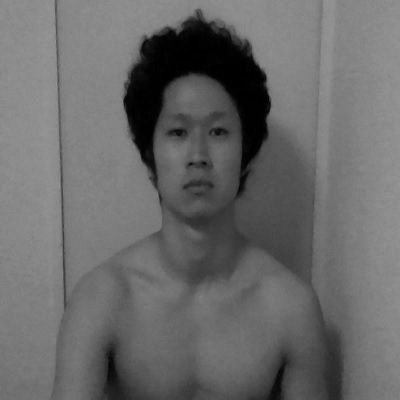
\includegraphics[width=30mm]{copied_bina_gray.jpg}
    \end{center}
    \caption{出力画像:Binary グレースケール画像}
    \label{fig:sutehage}
  \end{minipage}
\end{figure}

7-1b.
\begin{figure}[htbp]
  \begin{minipage}{0.25\hsize}
    \begin{center}
      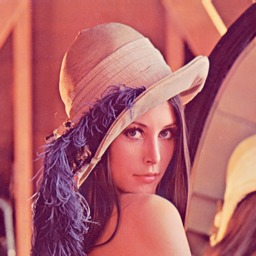
\includegraphics[width=30mm]{lenna256x256binary.jpg}
    \end{center}
    \caption{入力画像:カラー画像}
    \label{fig:sutehage}
  \end{minipage}
  \begin{minipage}{0.25\hsize}
    \begin{center}
      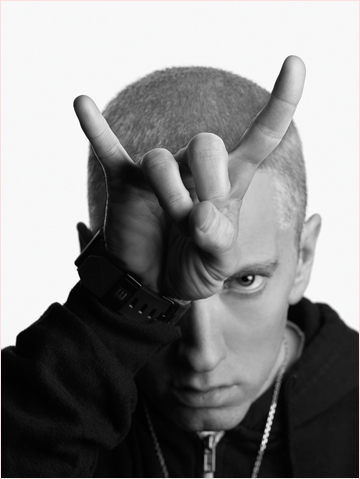
\includegraphics[width=30mm]{EMINEM_201310A.jpg}
    \end{center}
    \caption{入力画像:グレースケール画像}
    \label{fig:sutehage}
  \end{minipage}
  \begin{minipage}{0.25\hsize}
    \begin{center}
      
\includegraphics[width=30mm]{FilteredImageColor30.jpg}
    \end{center}

    \caption{出力画像:カラー画像30回フィルター}
    \label{fig:sutehage}
  \end{minipage}
  \begin{minipage}{0.25\hsize}
    \begin{center}
      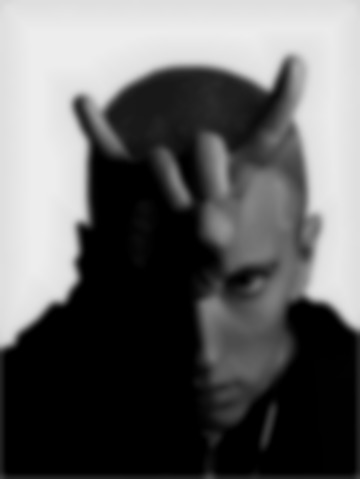
\includegraphics[width=30mm]{FilteredImageGray30.jpg}
    \end{center}
    \caption{出力画像:グレースケール画像30回フィルター}
    \label{fig:sutehage}
  \end{minipage}
\end{figure}
本当は70回フィルター、100回フィルターの結果も載せていたが、platexの際にオーバーフローを起こすとかバッファが足りないとか怒られて(! Unable to read an entire line---bufsize=200000.
  Please increase buf_size in texmf.cnf.
)のせることができなかった。ネットで検索したらsudoを使ってtexmf.cnの内部のbufsizeを書き換えたらいけるっぽかったけど、ルート権限になることができなかった。(s1811433@LC2RR-P010:~/prog2/07/07kadai$ sudo su -
  [sudo] s1811433 のパスワード:
残念ですが、ユーザー s1811433 は'/bin/su -' を root として LC2RR-P010.u.tsukuba.ac.jp 上で実行することは許可されていません。)
\begin{comment}

\begin{figure}[htbp]
  \begin{minipage}{0.25\hsize}
    \begin{center}
      \includegraphics[width=30mm]{FilteredImageColor70.jpg}
    \end{center}
    \caption{出力画像:カラー画像70回フィルター}
    \label{fig:sutehage}
  \end{minipage}
  \begin{minipage}{0.25\hsize}
    \begin{center}
      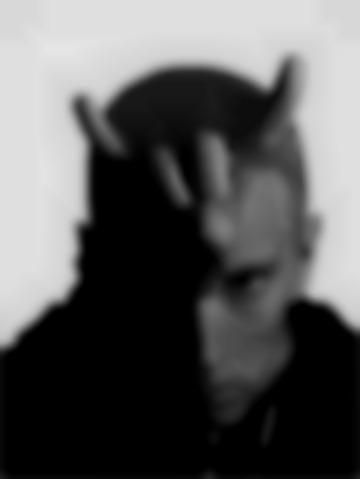
\includegraphics[width=30mm]{FilteredImageGray60.jpg}
    \end{center}
    \caption{出力画像:グレースケール画像60回フィルター}
    \label{fig:sutehage}
  \end{minipage}
  \begin{minipage}{0.25\hsize}
    \begin{center}
      
\includegraphics[width=30mm]{FilteredImageColor100.jpg}
    \end{center}

    \caption{出力画像:カラー画像100回フィルター}
    \label{fig:sutehage}
  \end{minipage}
  \begin{minipage}{0.25\hsize}
    \begin{center}
      
\includegraphics[width=30mm]{FilteredImageGray100.jpg}
    \end{center}
    \caption{出力画像:グレースケール画像100回フィルター}
    \label{fig:sutehage}
  \end{minipage}
\end{figure}

\end{comment}

\section{課題7-2}
\noindent a.
\subsection{source}
\lstinputlisting[basicstyle=\ttfamily\footnotesize,frame=single,breaklines=tr\
  ue,caption=Makefile2a]{Makefile2a}
\lstinputlisting[basicstyle=\ttfamily\footnotesize,frame=single,breaklines=tr\
  ue,caption=a7-2.c]{a7-2.c}
\lstinputlisting[basicstyle=\ttfamily\footnotesize,frame=single,breaklines=tr\
  ue,caption=headerB.h]{headerB.h}
\lstinputlisting[basicstyle=\ttfamily\footnotesize,frame=single,breaklines=tr\
  ue,caption=matrix.c]{matrix.c}
\lstinputlisting[basicstyle=\ttfamily\footnotesize,frame=single,breaklines=tr\
  ue,caption=vector.c]{vector.c}



\subsection{result}
\begin{lstlisting}[basicstyle=\ttfamily\footnotesize,frame=single,breaklines=tr\
  ue]
  s1811433@LC2RR-P010:~/prog2/07/07kadai$ make -f Makefile2a
  cc -o a7-2 a7-2.o matrix.o vector.o
  s1811433@LC2RR-P010:~/prog2/07/07kadai$ ./a7-2
  how's the scale of the matrix?: 2 2
  input the matrix's elements : 1 2 3 4

  matrix A:
  1.000000 2.000000
  3.000000 4.000000


  how's the scale of the vector?: 2
  input the vector's elements :
  1 2

  vector B:
  1.000000 2.000000

  AxB :
  5.000000 11.000000
  s1811433@LC2RR-P010:~/prog2/07/07kadai$ ./a7-2
  how's the scale of the matrix?: 2 3
  input the matrix's elements : 1 2 3 4 5 6

  matrix A:
  1.000000 2.000000 3.000000
  4.000000 5.000000 6.000000


  how's the scale of the vector?: 2
  input the vector's elements :
  1 2

  vector B:
  1.000000 2.000000 Can't multiply them!
  s1811433@LC2RR-P010:~/prog2/07/07kadai$ ./a7-2
  how's the scale of the matrix?: 2 3
  input the matrix's elements : 1 2 3 4 5 6

  matrix A:
  1.000000 2.000000 3.000000
  4.000000 5.000000 6.000000


  how's the scale of the vector?: 3
  input the vector's elements :
  1 2 3

  vector B:
  1.000000 2.000000 3.000000

  AxB :
  14.000000 26.000000 0.000000
  s1811433@LC2RR-P010:~/prog2/07/07kadai$
\end{lstlisting}



b.
\subsection{source}
\lstinputlisting[basicstyle=\ttfamily\footnotesize,frame=single,breaklines=tr\
  ue,caption=b7-2.c]{b7-2.c}
\lstinputlisting[basicstyle=\ttfamily\footnotesize,frame=single,breaklines=tr\
  ue,caption=linear.c]{linear.c}


\subsection{result}
\begin{lstlisting}[basicstyle=\ttfamily\footnotesize,frame=single,breaklines=tr\
    \
    ue]
  s1811433@LC2RR-P010:~/prog2/07/07kadai$ make -f Makefile2b -B
  cc -c b7-2.c headerB.h
  cc -c matrix.c
  cc -c vector.c
  cc -c linear.c headerB.h
  cc -o b7-2 b7-2.o matrix.o vector.o linear.o
  s1811433@LC2RR-P010:~/prog2/07/07kadai$ ./b7-2 data4x4.txt
  LoadLinerSystem: matrix size: 4x4


  Matrix A(4, 4)
  -7.000000 1.000000 -10.000000 -6.000000
  7.000000 5.000000 -9.000000 2.000000
  8.000000 5.000000 5.000000 3.000000
  -9.000000 8.000000 -7.000000 1.000000

  Vector b (4)
  2.000000 9.000000 8.000000 8.000000

  Answer: x(4)
  0.333525 1.363479 -0.067972 -0.381912

  Error: 0.000000
  s1811433@LC2RR-P010:~/prog2/07/07kadai$ ./b7-2 data10x10.txt
  LoadLinerSystem: matrix size: 10x10


  Matrix A(10, 10)
  -2.000000 2.000000 -7.000000 -7.000000 -7.000000 -1.000000 9.000000 9.000000 -5.000000 -9.000000
  -3.000000 -6.000000 6.000000 6.000000 2.000000 -4.000000 6.000000 -8.000000 6.000000 4.000000
  2.000000 9.000000 -8.000000 5.000000 3.000000 7.000000 -3.000000 1.000000 -2.000000 4.000000
  -9.000000 2.000000 2.000000 -2.000000 7.000000 -10.000000 1.000000 -1.000000 7.000000 4.000000
  1.000000 -4.000000 9.000000 2.000000 9.000000 -10.000000 7.000000 3.000000 -5.000000 4.000000
  -8.000000 -5.000000 -3.000000 4.000000 3.000000 5.000000 0.000000 6.000000 7.000000 7.000000
  6.000000 9.000000 2.000000 -2.000000 1.000000 9.000000 1.000000 6.000000 -9.000000 -5.000000
  2.000000 6.000000 8.000000 6.000000 1.000000 7.000000 6.000000 9.000000 -3.000000 1.000000
  -8.000000 2.000000 1.000000 -8.000000 -3.000000 -8.000000 -6.000000 4.000000 9.000000 -3.000000
  -6.000000 5.000000 -8.000000 -4.000000 7.000000 -3.000000 5.000000 9.000000 5.000000 1.000000

  Vector b (10)
  9.000000 -4.000000 -9.000000 9.000000 2.000000 -10.000000 -2.000000 -4.000000 -2.000000 -7.000000

  Answer: x(10)
  2.385402 2.742281 2.022468 -12.917047 -7.374715 1.773511 5.067214 -2.236396 -1.366858 16.681884

  Error: 0.000000
  s1811433@LC2RR-P010:~/prog2/07/07kadai$
  
\end{lstlisting}





\begin{comment}
\section{課題1-3}
\subsection{source}
\lstinputlisting[basicstyle=\ttfamily\footnotesize,frame=single,breaklines=tr\
ue,caption=]{a1-3.c}

\subsection{result}

\begin{lstlisting}[basicstyle=\ttfamily\footnotesize,frame=single,breaklines=tr\
  ue,caption=]
  
\end{lstlisting}

\begin{figure}[h]
  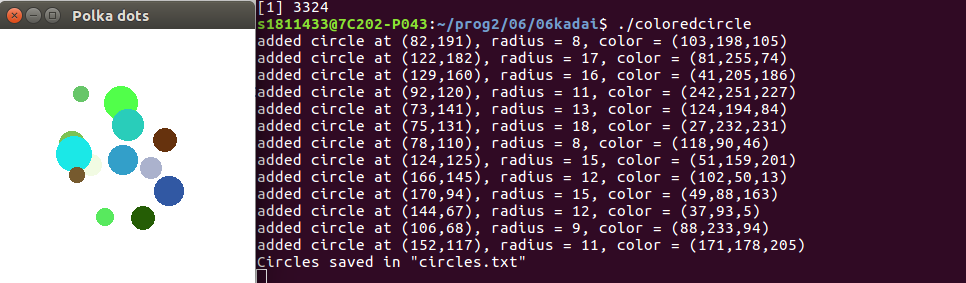
\includegraphics[width=0.8\linewidth]{b.png}
  \caption{数回クリックしたあとにsを押した}
  \label{fig:sutehage}
\end{figure}  
\end{comment}


\end{document}
